% \documentclass[usenames, dvipsnames, t, table, handout]{beamer}
\documentclass[usenames, dvipsnames, t, table]{beamer}
% === BEAMER AND FORMATTING STUFF ===

\usetheme{default}
\usefonttheme{structurebold}
\setbeamertemplate{navigation symbols}{}
% \setbeamertemplate{footline}[frame number]

% Unnumbered footnote with no rule.
\renewcommand*\footnoterule{}%
\newcommand\unnumberedfootnote[1]{%
  \begingroup
  \renewcommand\thefootnote{}\footnote{#1}%
  \addtocounter{footnote}{-1}%
  \endgroup
}

\usepackage{tikz}
\usetikzlibrary{arrows.meta}
\usetikzlibrary{calc}
\usetikzlibrary{positioning}

\let\OLDitemize\itemize
\renewcommand\itemize{\OLDitemize\addtolength{\itemsep}{5pt}}

\newcommand{\inlineauthor}[1]{\raisebox{-0.5 \height}{\includegraphics[height=1cm]{assets/#1}}}

% \setbeamercovered{transparent}

% \usepackage[table]{xcolor}

% === PACKAGES ===
% For some reason I have to leave this in to use ifthenelse????? even though I'm not even compiling with pythontex???? This makes negative sense. But, no time to understand it now.
% \usepackage{pythontex}
\usepackage{multicol}
\usepackage{makecell}
\usepackage{url}
\usepackage{ifthen}

% === MATH STUFF ===
\newcommand{\A}{\mathcal{A}}
\renewcommand{\P}{\mathcal{P}}
\newcommand{\eps}{\epsilon}

% % === CUSTOM TIKZ ===

% \newcommand{\cycle}{
%   \foreach \t in {0, ...,\n}{
%     \pgfmathparse{int(Mod(\t, \spacing))}
%     \ifthenelse{\pgfmathresult=1}{
%       \node[roundnode,  draw=orange!60, fill=orange!5] (c\t) at ({\x + \scale *
%         cos(360 * (\t / (\n + 1)))}, {\y + \scale * sin(360 *
%         (\t / (\n + 1))}) {};
%     }
%     {
%         \node[roundnode] (c\t) at ({\x + \scale * cos(360 * (\t /
%         (\n + 1)))}, {\y + \scale * sin(360 * (\t / (\n + 1))})
%         {};
%     }

%   \pgfmathparse{int(\n - 1)}
%   \foreach \t in {0, ..., \pgfmathresult}{
%     \pgfmathparse{int(\t + 1)}]
%     \draw[-Latex] (c\t) -- (c\pgfmathresult);
%     }
%   }
%   \draw[-Latex] (c\n) -- (c0) node[midway, right] {$f$};
% }

% \newcommand{\plaincycle}{
%   \foreach \t in {0, ...,\n}{
%       \node[roundnode] (pc\t) at ({\x + \scale *
%         cos(360 * (\t / (\n + 1)))}, {\y + \scale * sin(360 *
%         (\t / (\n + 1))}) {};
%   }

%   \pgfmathparse{int(\n - 1)}
%   \foreach \t in {0, ..., \pgfmathresult}{
%     \pgfmathparse{int(\t + 1)}]
%     \draw[-Latex] (pc\t) -- (pc\pgfmathresult);
%   }
%   \draw[-Latex] (pc\n) -- (pc0) node[midway, right] {$f$};
% }

% % \newcommand{\points}[1]{
% %     \node[roundnode] (1) at (#1, 0) {1};
% %     \node[roundnode, anchor=north] (2) at (1.south) {2};
% %     \node[roundnode, anchor=north] (3) at (2.south) {3};
% %     \node[roundnode, below=0.6cm] (4) at (3.south) {$N$};
% %     \path (3) -- node[auto=false]{\vdots} (4);

% %     \node[roundnode] (A) at ({#1 + 2}, 0) {1};
% %     \node[roundnode, anchor=north] (B) at (A.south) {2};
% %     \node[roundnode, anchor=north] (C) at (B.south) {3};
% %     \node[roundnode, below=0.6cm] (D) at (C.south) {$N$};
% %     \path (C) -- node[auto=false]{\vdots} (D);
% %   }

%   \newcommand{\halfpoints}[1]{
%     \node[roundnode] (1) at (#1, 0) {1};
%     \node[roundnode, anchor=north] (2) at (1.south) {2};
%     \node[roundnode, below=0.3cm] (3) at (2.south) {74};
%     \path (2) -- node[auto=false]{\small{\vdots}} (3);
%     \node[roundnode, below=0.3cm] (4) at (3.south) {$N$};
%     \path (3) -- node[auto=false]{\small{\vdots}} (4);
%     \node[roundnode, below=0.3cm] (3) at (2.south) {74};
%     \node[roundnode, below=0.3cm] (4) at (3.south) {$N$};

%     % \node[] (A) at ({#1 + 2}, 0) {1};
%     % \node[anchor=north] (B) at (A.south) {};
%     % \node[anchor=north] (C) at (B.south) {};
%     % \node[below=0.6cm] (D) at (C.south) {};
%     % \path (C) -- node[auto=false]{\vdots} (D);
%     }

% %       \newcommand{\roundnode}{roundnode/.style={circle, draw=green!60, fill=green!5, very thick, minimum size=5mm}}
% === CUSTOM TIKZ ===

\newcommand{\cycle}{
  \foreach \t in {0, ...,\n}{
    \pgfmathparse{int(Mod(\t, \spacing))}
    \ifthenelse{\pgfmathresult=1}{
      \node[roundnode,  draw=orange!60, fill=orange!5] (\t) at ({\x + \scale *
        cos(360 * (\t / (\n + 1)))}, {\y + \scale * sin(360 *
        (\t / (\n + 1))}) {};
    }{
      \node[roundnode] (\t) at ({\x + \scale * cos(360 * (\t /
        (\n + 1)))}, {\y + \scale * sin(360 * (\t / (\n + 1))})
        {};
    }

  }

  \pgfmathparse{int(\n - 1)}
  \foreach \t in {0, ..., \pgfmathresult}{
    \pgfmathparse{int(\t + 1)}]
    \draw[-Latex] (\t) -- (\pgfmathresult);
  }
  \draw[-Latex] (\n) -- (0) node[midway, right] {$f$};
}

\newcommand{\plaincycle}{
  \foreach \t in {0, ...,\n}{
      \node[roundnode] (\t) at ({\x + \scale *
        cos(360 * (\t / (\n + 1)))}, {\y + \scale * sin(360 *
        (\t / (\n + 1))}) {};
  }

  \pgfmathparse{int(\n - 1)}
  \foreach \t in {0, ..., \pgfmathresult}{
    \pgfmathparse{int(\t + 1)}]
    \draw[-Latex] (\t) -- (\pgfmathresult);
  }
  \draw[-Latex] (\n) -- (0) node[midway, right] {$f$};
}

% \newcommand{\points}[1]{
%     \node[roundnode] (1) at (#1, 0) {1};
%     \node[roundnode, anchor=north] (2) at (1.south) {2};
%     \node[roundnode, anchor=north] (3) at (2.south) {3};
%     \node[roundnode, below=0.6cm] (4) at (3.south) {$N$};
%     \path (3) -- node[auto=false]{\vdots} (4);

%     \node[roundnode] (A) at ({#1 + 2}, 0) {1};
%     \node[roundnode, anchor=north] (B) at (A.south) {2};
%     \node[roundnode, anchor=north] (C) at (B.south) {3};
%     \node[roundnode, below=0.6cm] (D) at (C.south) {$N$};
%     \path (C) -- node[auto=false]{\vdots} (D);
%   }

  \newcommand{\halfpoints}[1]{
    \node[roundnode] (1) at (#1, 0) {1};
    \node[roundnode, anchor=north] (2) at (1.south) {2};
    \node[roundnode, below=0.3cm] (3) at (2.south) {74};
    \path (2) -- node[auto=false]{\small{\vdots}} (3);
    \node[roundnode, below=0.3cm] (4) at (3.south) {$N$};
    \path (3) -- node[auto=false]{\small{\vdots}} (4);
    \node[roundnode, below=0.3cm] (3) at (2.south) {74};
    \node[roundnode, below=0.3cm] (4) at (3.south) {$N$};

    % \node[] (A) at ({#1 + 2}, 0) {1};
    % \node[anchor=north] (B) at (A.south) {};
    % \node[anchor=north] (C) at (B.south) {};
    % \node[below=0.6cm] (D) at (C.south) {};
    % \path (C) -- node[auto=false]{\vdots} (D);
    }

% \newcommand{\roundnode}{roundnode/.style={circle, draw=green!60, fill=green!5, very thick, minimum size=5mm}}


% === BODY ===

\title{Revisiting Time-Space Tradeoffs for Function Inversion}
% \author{\textbf{Spencer Peters \newline  \scriptsize{May 16, 2022}}}
% \author{\textbf{Spencer Peters} \newline \newline \scriptsize{Joint with}}
\author{\textbf{Spencer Peters}}
% \institute{Cornell University}
\date{}

\begin{document}

%
\newcommand{\mypause}{\par\pause\noindent}

% Preprint reference
\nocite{FIPreprint}

% \renewcommand{\pause}{}
% \renewcommand{\mypause}{}
% \renewcommand{\only}{}


\begin{frame}
  \vspace{1em}
  \titlepage
  \begin{tikzpicture}[remember picture, overlay]
    \node[anchor = south west] (A)  at ($(current page.south west) + (2.75, 0.5) $){
        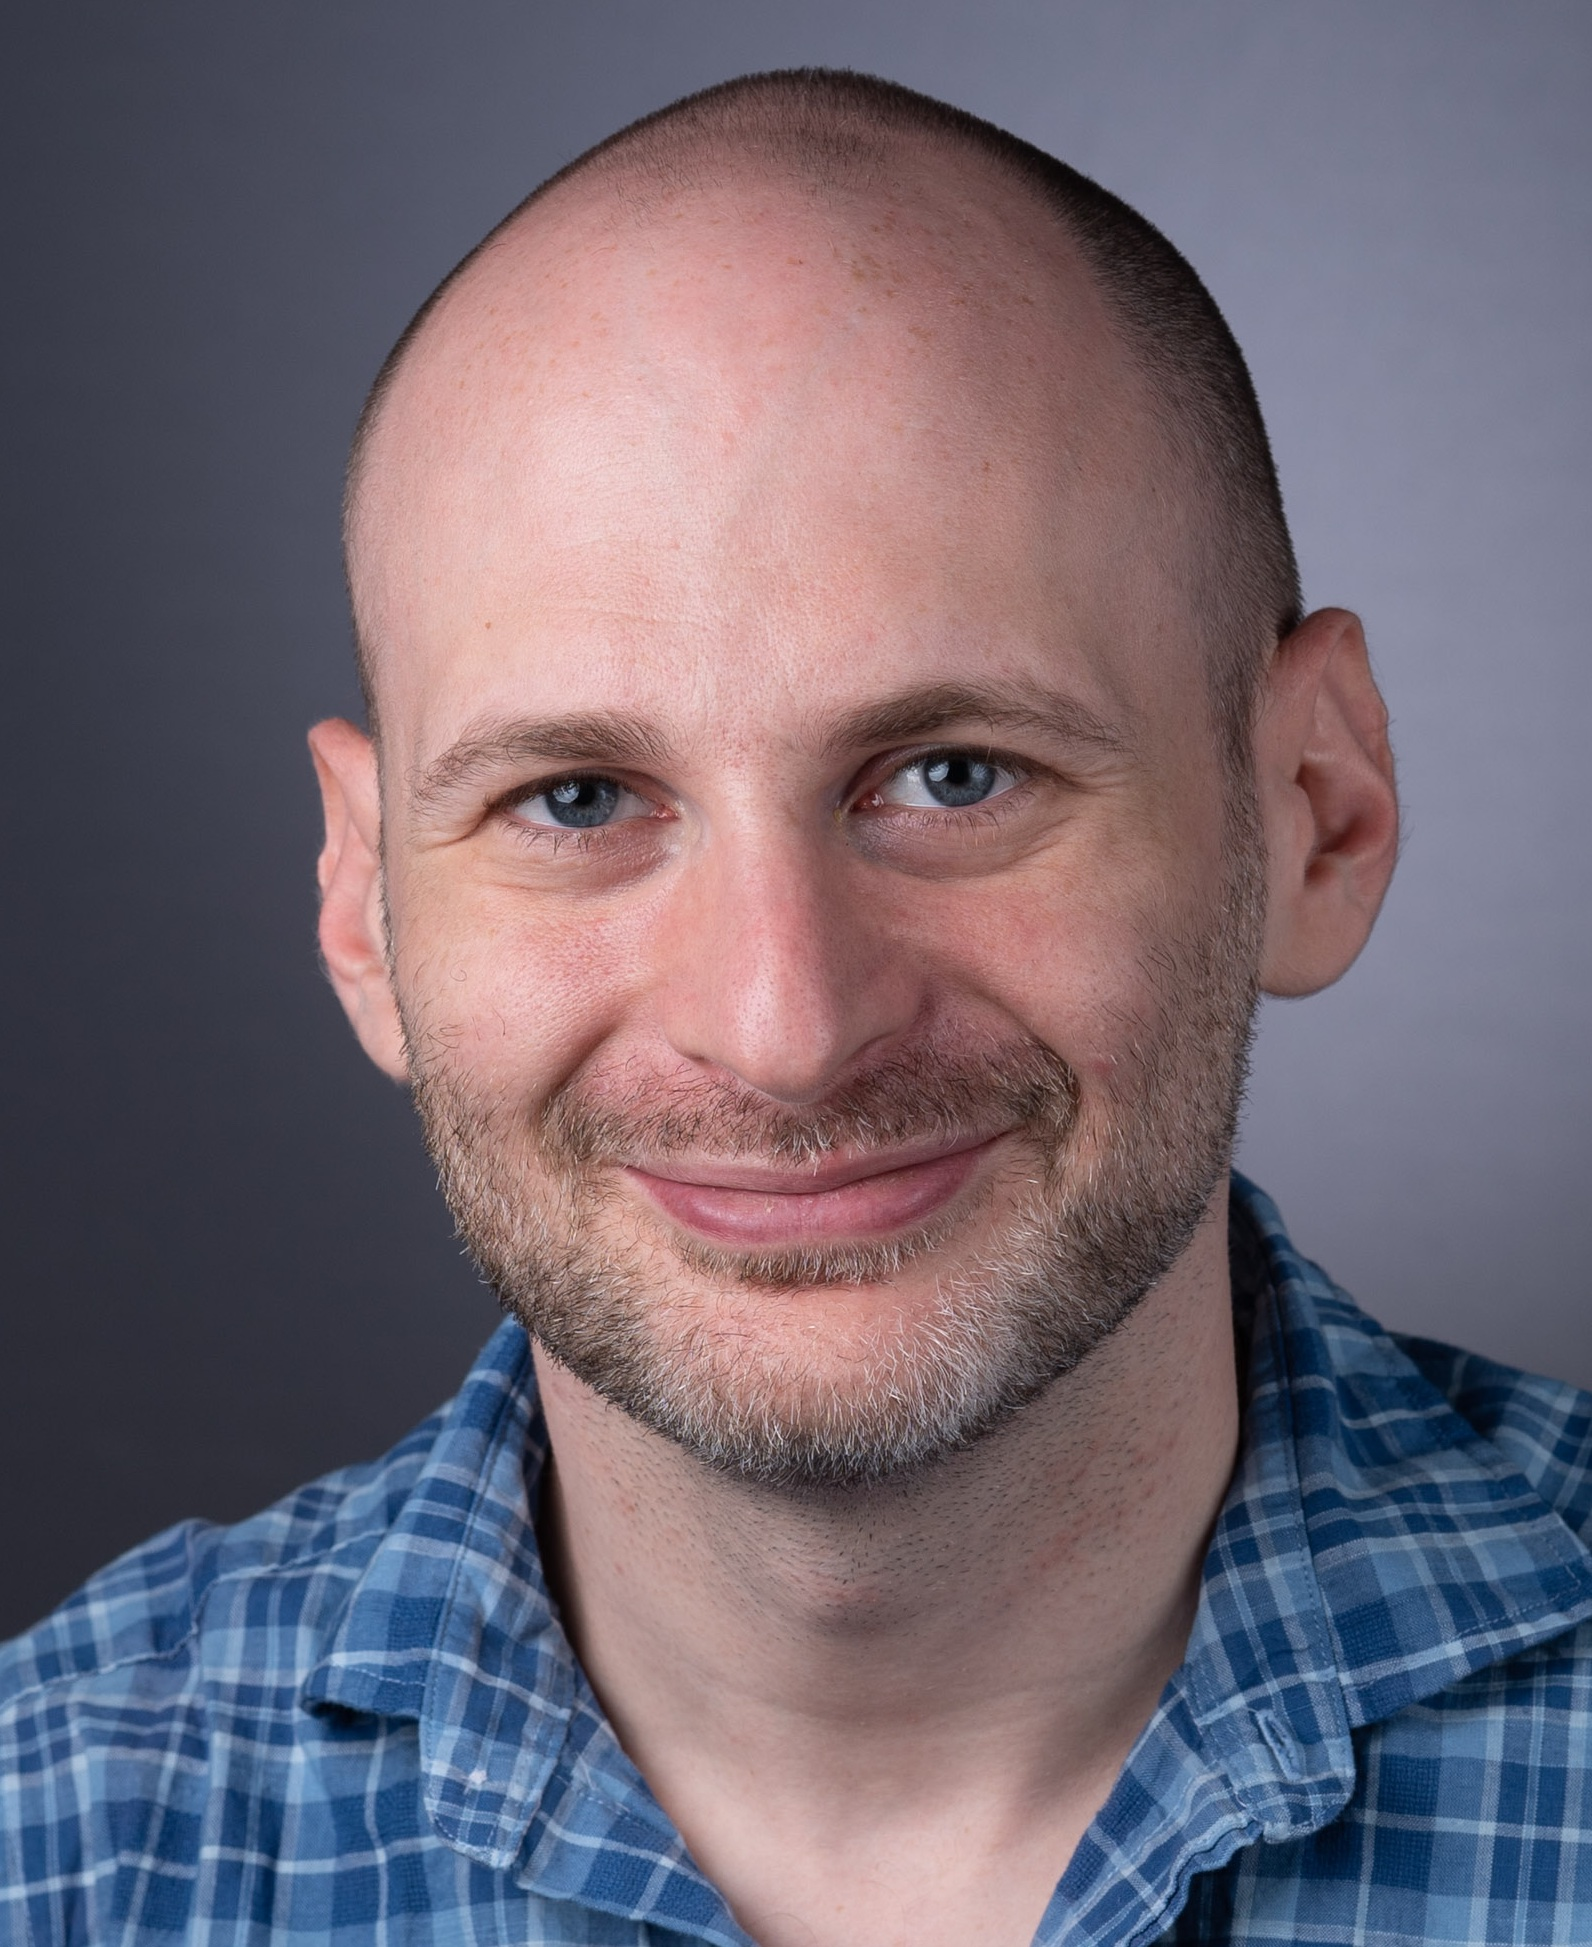
\includegraphics[height=3cm]{assets/noah.jpeg}
      };
      \node[anchor = west] (B) at (A.east){
        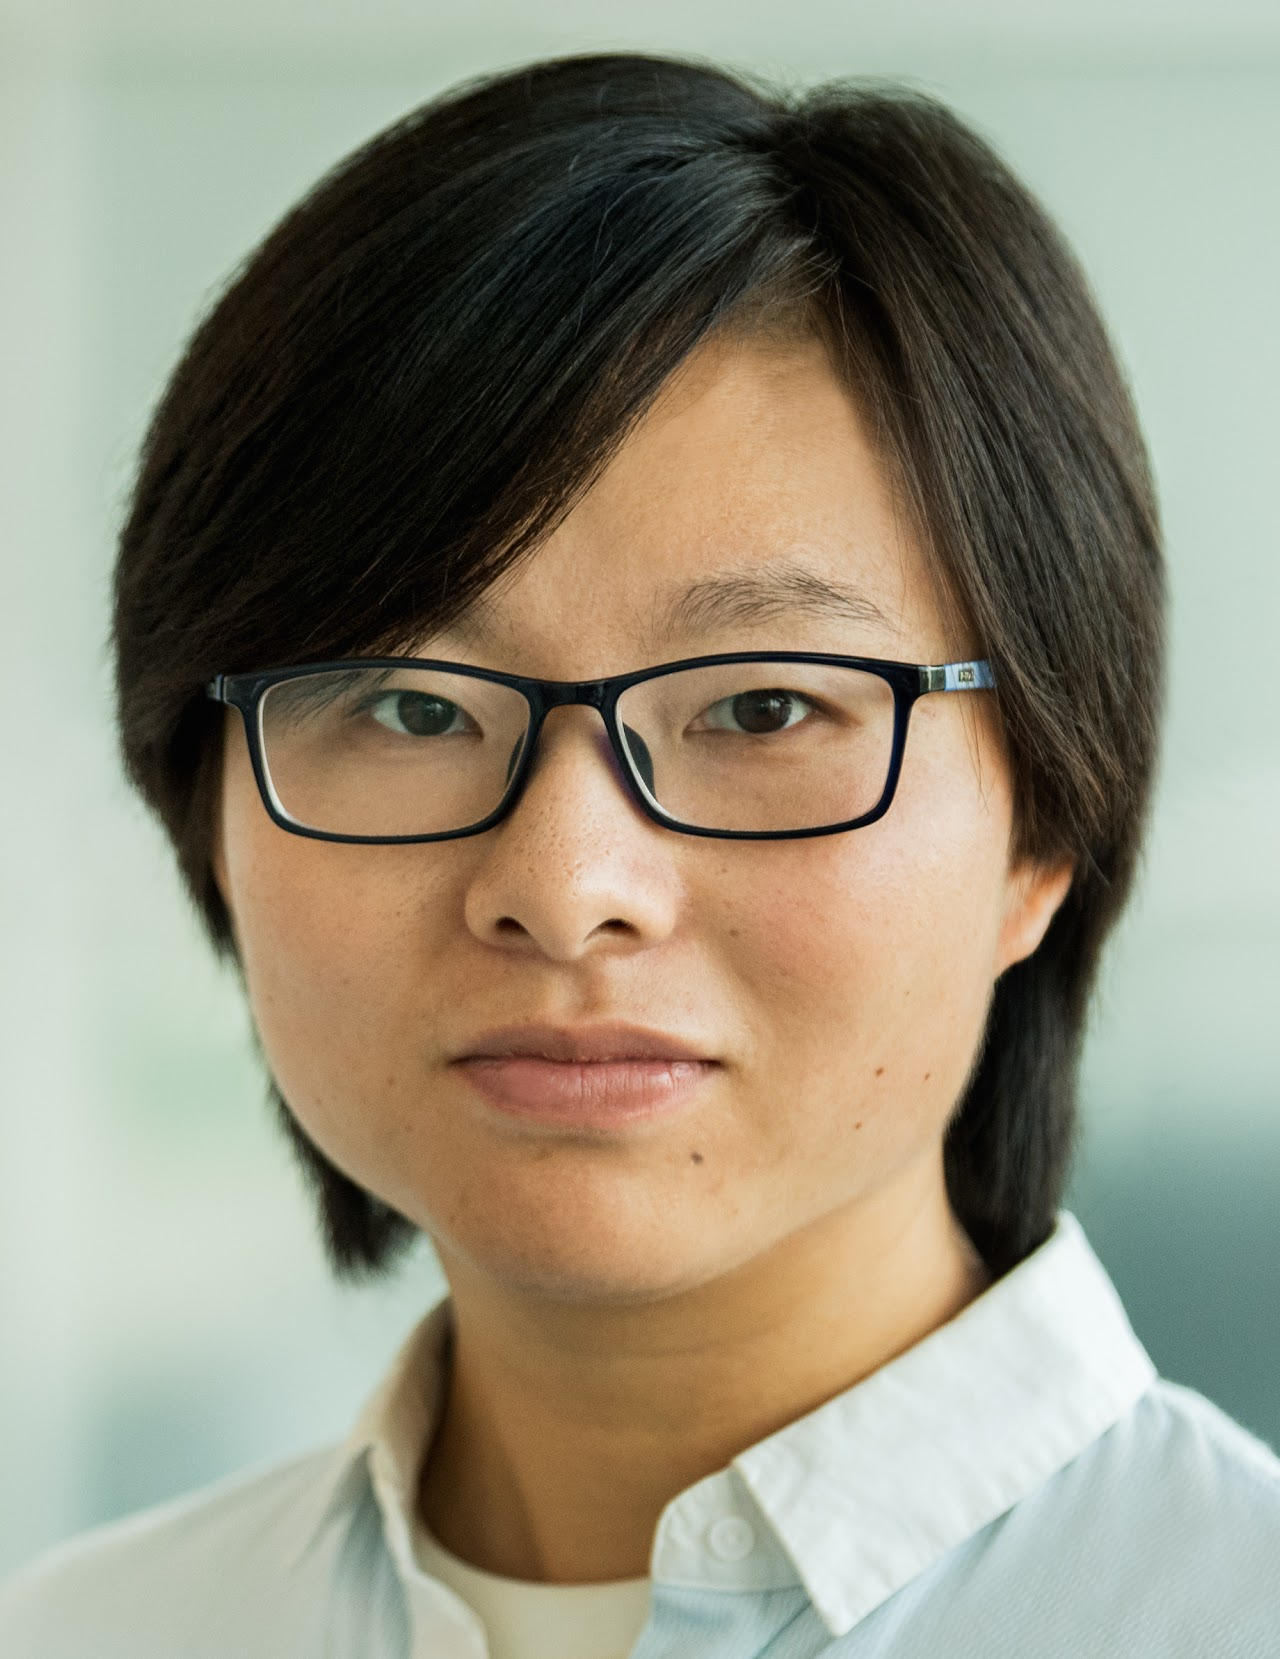
\includegraphics[height=3cm]{assets/siyao.jpeg}
      };
          \node[anchor = west] (C) at (B.east){
        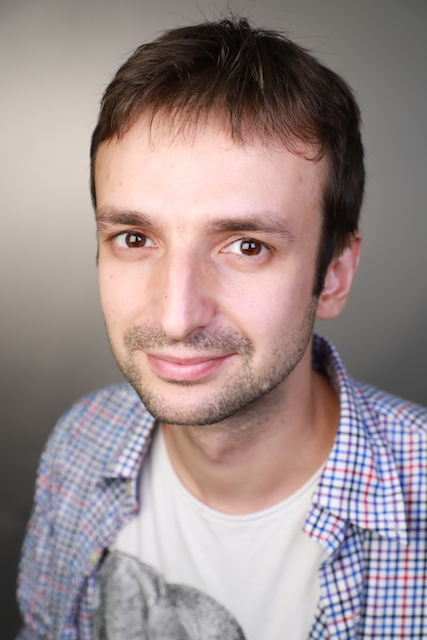
\includegraphics[height=3cm]{assets/sasha.jpeg}
      };

      % \node[align=left] (AA) at (A.north) {\scriptsize{Noah \\ Stephens-Davidowitz}};
      \node[align=center] (AA) at (A.north) {\scriptsize{Noah S.D.}};
      \node[align=center] (BB) at (B.north) {\scriptsize{Siyao Guo}};
      \node[align=center] (CC) at (C.north) {\scriptsize{Sasha Golovnev}};


      \node[anchor = north] (CornellCS) at (current page.north) {
        
\includegraphics[height = 1.5cm]{assets/cornell.png}
        };
  \end{tikzpicture}
\end{frame}

\begin{frame}
  \frametitle{Function Inversion}
  \begin{itemize}
  \item Given a function $f: \{1, 2, \dots, N\} \to \{1, 2, \dots, N\}$ and a point $y$ in its image, find $x$ with $f(x) = y$.
  \end{itemize}
\end{frame}

\begin{frame}
  \frametitle{Function Inversion}
  \vspace{-0.45cm}
  \begin{itemize}
  \item Given a function $f: \{1, 2, \dots, N\} \to \overbrace{\{1, 2, \dots, N\}}^{[N]}$ and a point $y$ in its image, find $x$ with $f(x) = y$.
    % from a discrete set to itself (say, a cryptographic hash function), and a point $y$ in the range, how do I invert?
  \end{itemize}
  \pause
  \hspace{5em}
  \scalebox{0.8}{
    \begin{tikzpicture}[roundnode/.style={circle, draw=green!60, fill=green!5, very thick, minimum size=3mm}]
    % \points{2}

    % \only<2->{
    % \draw[-Latex] (1.east) -- node[midway, above] {$f$} (B.west);
    % \draw[-Latex] (2.east) -- (C.west);
    % \draw[-Latex] (3.east) -- (C.west);
    % \draw[-Latex] (4.east) -- (A.west);
    % }

    % \only<3->{
    % \node[roundnode, anchor=north, draw=red!60, fill=red!5] (C) at (B.south) {3};}
    % \only<4->{
    % \node[roundnode, anchor=north, draw=blue!60, fill=blue!5] (2) at (1.south) {2};}

    % \only<9>{
    %   \points{7}

    % \draw[-Latex] (1.east) -- node[midway, above] {$f$} (B.west);
    % \draw[-Latex] (2.east) -- (D.west);
    % \draw[-Latex] (3.east) -- (C.west);
    % \draw[-Latex] (4.east) -- (A.west);
    %   }
      % \newcommand{\mydraw}[2]{
      %   \draw[-Latex] #1 .. controls ($0.5 * #1 + 0.5 * #2 + (1, 0)$) .. #2;
      % }

      % ===
    %   \halfpoints{2}
    %   \only<2->{
    %         \draw[-Latex] (1.east) .. controls ($0.5*(1.east) + 0.5*(2.east) + (1, 0)$) .. node[midway, right] {$f$} (2.east);
    %         % \draw[-Latex] (2.east) .. controls (3, -1.5) .. (3.east);
    %         \draw[-Latex] (2.east) .. controls ($0.5*(2.east) + 0.5*(3.east) + (1, 0)$) .. (3.east);
    %         % \draw[-Latex] (3.east) .. controls (3, -1.5) and (3, -2.5) .. (3.east);
    %         \draw[-Latex] (3.west) .. controls ($0.5*(3.west) + 0.5*(3.west) + (-0.75, 0.5)$) and ($0.5*(3.west) + 0.5*(3.west) + (-0.75, -0.5)$) .. (3.west);
    %         % \draw[-Latex] (4.east) .. controls (3, -2.5) .. (1.east);
    %        \draw[-Latex] (4.west) .. controls ($0.5*(4.west) + 0.5*(1.west) + (-1, 0)$) ..  (1.west);

    %      }

    %      \only<3->{
    % \node[roundnode, anchor=north, draw=red!60, fill=red!5] (3) at (2.south) {3};}
    % \only<4->{
    %   \node[roundnode, anchor=north, draw=blue!60, fill=blue!5] (2) at (1.south) {2};}

    %    \only<9>{
    %   \halfpoints{7}
    % \draw[-Latex] (1.east) .. controls ($0.5*(1.east) + 0.5*(3.east) + (1, 0)$) .. node[midway, right] {$f$} (3.east);
    % \draw[-Latex] (3.east) .. controls ($0.5*(3.east) + 0.5*(4.east) + (1, 0)$) .. (4.east);
    % \draw[-Latex] (2.west) .. controls ($0.5*(2.west) + 0.5*(2.west) + (-0.75, 0.5)$) and ($0.5*(2.west) + 0.5*(2.west) + (-0.75, -0.5)$) .. (2.west);
    % \draw[-Latex] (4.west) .. controls ($0.5*(4.west) + 0.5*(1.west) + (-1, 0)$) ..  (1.west);
    % ===
            \halfpoints{2}
      \only<2->{
            \draw[-Latex] (1.east) .. controls ($0.5*(1.east) + 0.5*(2.east) + (1, 0)$) .. node[midway, right] {$f$} (2.east);
            % \draw[-Latex] (2.east) .. controls (3, -1.5) .. (3.east);
            \draw[-Latex] (2.east) .. controls ($0.5*(2.east) + 0.5*(3.east) + (1, 0)$) .. (3.east);
            % \draw[-Latex] (3.east) .. controls (3, -1.5) and (3, -2.5) .. (3.east);
            \draw[-Latex] (3.west) .. controls ($0.5*(3.west) + 0.5*(3.west) + (-0.75, 0.5)$) and ($0.5*(3.west) + 0.5*(3.west) + (-0.75, -0.5)$) .. (3.west);
            % \draw[-Latex] (4.east) .. controls (3, -2.5) .. (1.east);
           \draw[-Latex] (4.west) .. controls ($0.5*(4.west) + 0.5*(2.west) + (-1, 0)$) ..  (2.west);

         }

         \only<3->{
    \node[roundnode, below=0.3cm, draw=red!60, fill=red!5] (3) at (2.south) {74};}
    \only<4->{
      \node[roundnode, anchor=north, draw=blue!60, fill=blue!5] (2) at (1.south) {2};}

       \only<8>{
      \halfpoints{7}
    \draw[-Latex] (1.east) .. controls ($0.5*(1.east) + 0.5*(3.east) + (1, 0)$) .. node[midway, right] {$f$} (3.east);
    \draw[-Latex] (3.east) .. controls ($0.5*(3.east) + 0.5*(4.east) + (1, 0)$) .. (4.east);
    \draw[-Latex] (2.west) .. controls ($0.5*(2.west) + 0.5*(2.west) + (-0.75, 0.5)$) and ($0.5*(2.west) + 0.5*(2.west) + (-0.75, -0.5)$) .. (2.west);
    \draw[-Latex] (4.west) .. controls ($0.5*(4.west) + 0.5*(1.west) + (-1, 0)$) ..  (1.west);
    }

    \end{tikzpicture}}
\only<5->{
  \begin{itemize}
    \item We're interested in algorithms that invert any function, using only the ability to evaluate it.
    % \item This is a basic problem with many applications.
  % \only<6->{\item Codebreakers and mathematicians have been inverting specific functions for centuries.}
    \only<6->{\item The study of this \emph{black-box} function inversion problem was initiated by Martin Hellman \raisebox{-0.5 \height}{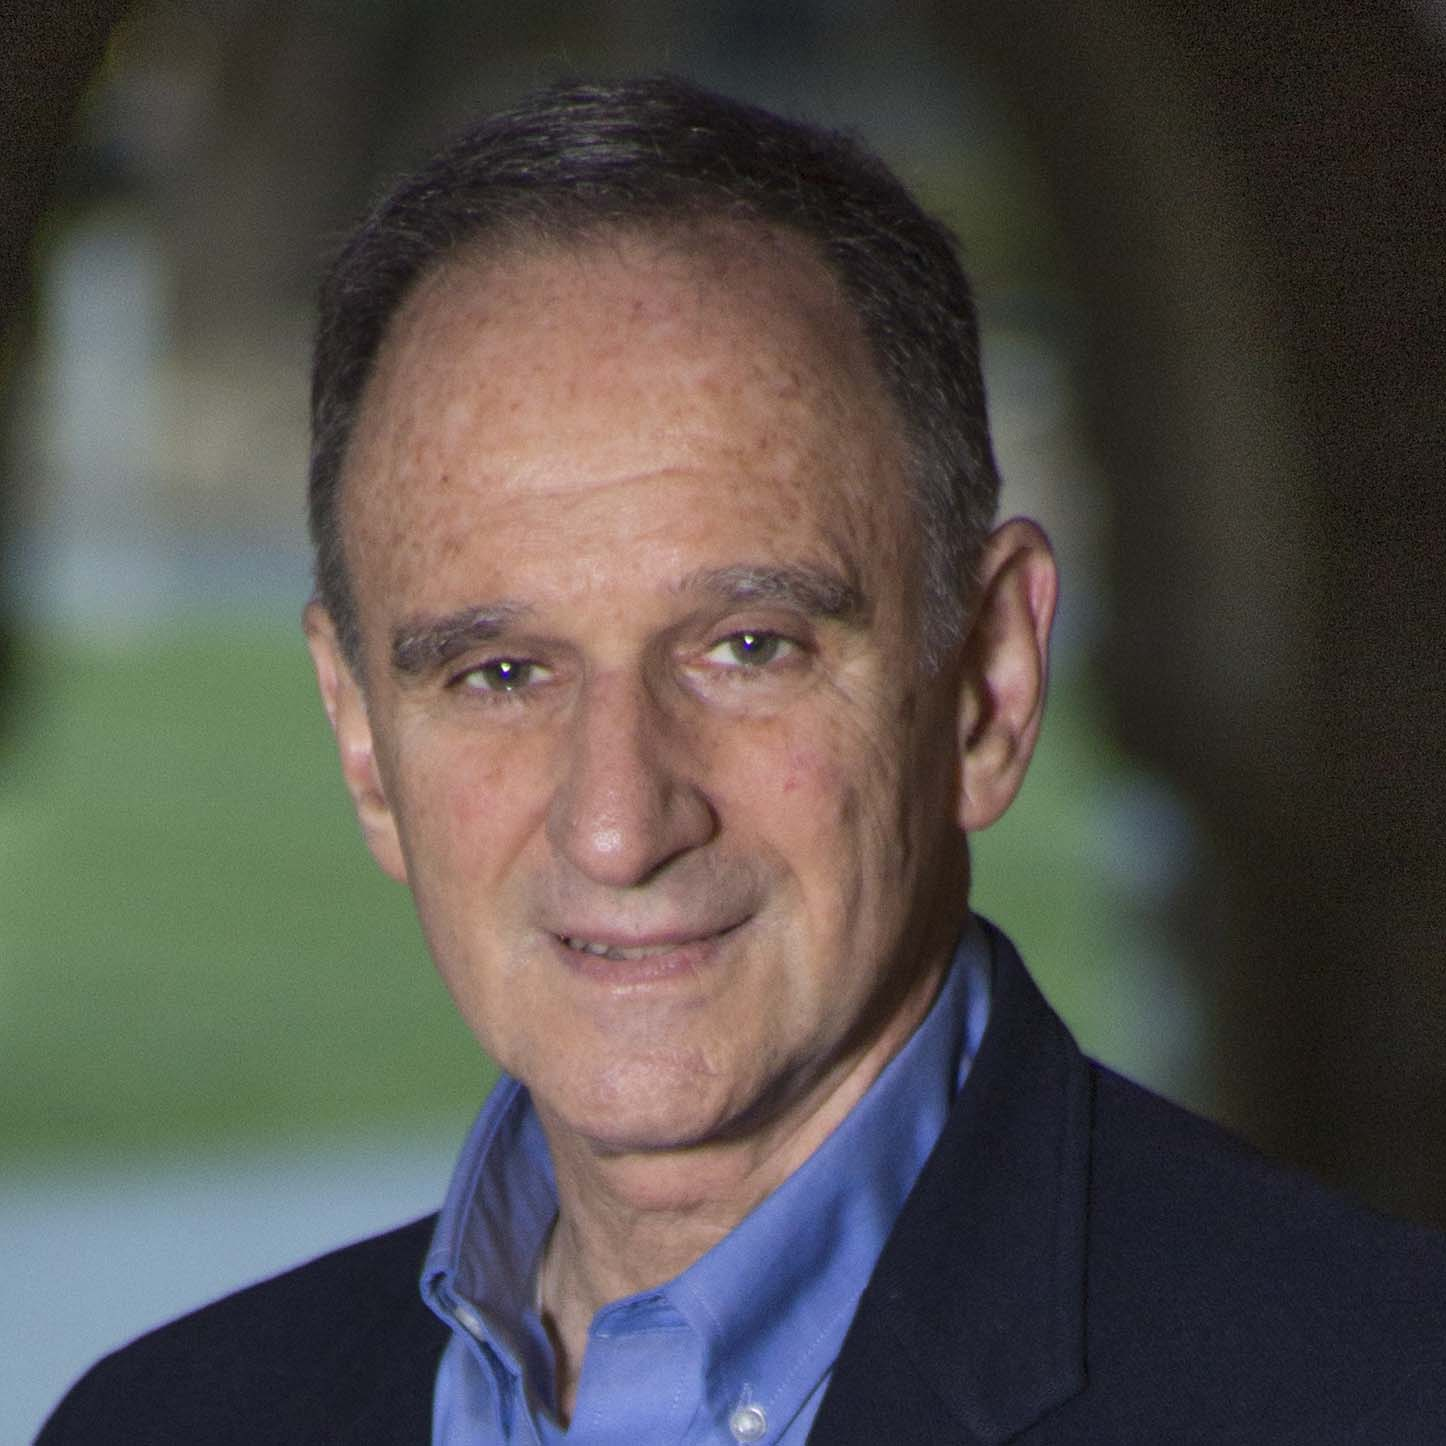
\includegraphics[height=1cm]{assets/hellman.jpeg}} in 1980 \cite{Hellman80}.}
    % \only<6->{\item Hellman's algorithm for permutations is beautiful and illustrative.}
    \only<7->{\item The algorithm Hellman devised is beautiful, and for the special case of permutations, quite simple.}
    % NOTE emphasize algorithm is beautiful
    % NOTE algorithm will notivate model
    % \pause
  % \item Hellman gave ``time-space tradeoffs'' for inverting permutations and inverting a randomly chosen function.
    % For example, f is a cryptographic hash function. We're trying to recover a password from its stored hash.
    % We're trying to forge a document with a given checksum/fingerprint ("hash").
  \end{itemize}}
\end{frame}

% \begin{frame}
%   \frametitle{Function Inversion}
%   \begin{itemize}
%   %It's better to see the algorithm before I tell you what that means.
%   \end{itemize}
% \end{frame}


  \begin{frame}
    \frametitle{Hellman's algorithm}
    \begin{itemize}
    \item If $f$ is a permutation, its \emph{graph} is a disjoint union of cycles.
    \end{itemize}
    \pause
      \vspace{1ex}

    % LATER animate these!
    \scalebox{0.8}{
    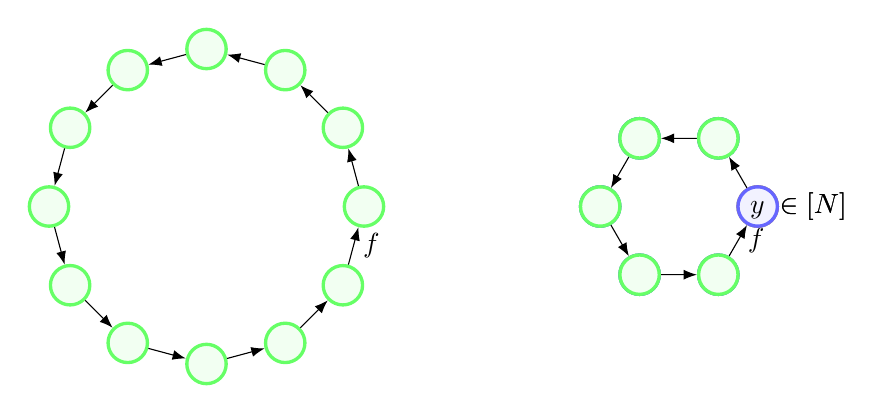
\begin{tikzpicture}[roundnode/.style={circle, draw=green!60, fill=green!5, very thick, minimum size=5mm}]
       \newcommand{\spacing}{3}
       \newcommand{\n}{11}
       \newcommand{\scale}{2}
       \newcommand{\x}{1}
       \newcommand{\y}{-1}
       \plaincycle

       \renewcommand{\spacing}{3}
       \renewcommand{\n}{5}
       \renewcommand{\scale}{1}
       \renewcommand{\x}{7}
       \renewcommand{\y}{-1}
       \plaincycle
       % \node [right=-0.03cm of 0.west] {$y \in [N]$};
       \node<3->[roundnode, draw=purple!60, fill=purple!5] at (0) {};
       % \node<3-> [right=0.05cm of 0.west] {$y \; \in [N] := \{1, 2, \dots, N\}$};
       \node<3-> [right=0.05cm of 0.west] {$y \; \in [N]$};
       % \pause
       % \node[roundnode, draw=purple!60, fill=purple!5] at (0) {};
       % \node[right=0.05cm of 0.west] {$y \; \in [N] := \{1, 2, \dots, N\}$};
       \node<6->[roundnode, draw=blue!60, fill=blue!5] at (1) {};
       \node<7->[roundnode] at (1) {};
       \node<7->[roundnode, draw=blue!60, fill=blue!5] at (2) {};
              \node<8->[roundnode] at (2) {};
       \node<8->[roundnode, draw=blue!60, fill=blue!5] at (3) {};
              \node<9->[roundnode] at (3) {};
              \node<9->[roundnode, draw=blue!60, fill=blue!5] at (4) {};
                     \node<10->[roundnode] at (4) {};

                     \node<10->[roundnode, draw=blue!60, fill=blue!5] at (5) {};
                            \node<11->[roundnode] at (5) {};

                            \node<11->[roundnode, draw=blue!60, fill=blue!5] at (0) {};
                            \node<11-> [right=0.05cm of 0.west] {$y \; \in [N]$};

     \end{tikzpicture}}
   \pause
   \pause

   \begin{itemize}
   \item Starting point: Hope $y$ is on a small cycle.
     \pause
   \item Compute $f(y)$, $f(f(y))$, and so on until you reach $y$ again.
     \pause
     \only<12>{\item Of course, $y$ might not be on a small cycle...}
     \end{itemize}
   \end{frame}

     \begin{frame}
    \frametitle{Hellman's algorithm}
    \begin{itemize}
    \item What if $y$ is on a large cycle?
      \end{itemize}
    \vspace{1ex}

    \scalebox{0.8}{
      \begin{tikzpicture}[roundnode/.style={circle, draw=green!60, fill=green!5, very thick, minimum size=5mm}]
       % \newcommand{\spacing}{3}
       % \newcommand{\n}{11}
       % \newcommand{\scale}{2}
       % \newcommand{\x}{1}
       % \newcommand{\y}{-1}
       % \only<2, 3>{\plaincycle}
       % \only<4->{\cycle}
       % \node<3, 5->[roundnode, draw=purple!60, fill=purple!5] at (0) {};
       % \node<3, 5-> [right=0.05cm of 0.west] {$y \; \in [N]$};
       % \only<7-> \draw[-Latex, color=orange] (1) -- (10);

       \newcommand{\spacing}{3}
       \newcommand{\n}{5}
       \newcommand{\scale}{1}
       \newcommand{\x}{7}
       \newcommand{\y}{-1}
       \only<2, 3>{\plaincycle}
       \only<4->{\cycle}

       \renewcommand{\spacing}{3}
       \renewcommand{\n}{11}
       \renewcommand{\scale}{2}
       \renewcommand{\x}{1}
       \renewcommand{\y}{-1}
       \only<2, 3>{\plaincycle}
       \only<4->{\cycle}
       \node<3, 5->[roundnode, draw=purple!60, fill=purple!5] at (0) {};
       \node<3, 5-> [right=0.05cm of 0.west] {$y \; \in [N]$};

       \only<6->{\node[roundnode, draw=blue!60, fill=orange!5] at (1) {};}
       \only<8-> \draw[-Latex, color=orange] (1) -- (10);
       \only<9->{\node[roundnode, draw=orange!60, fill=orange!5] at (1) {};}
       \only<9->{\node[roundnode, draw=blue!60, fill=orange!5] at (10) {};}
       \only<10->{\node[roundnode, draw=orange!60, fill=orange!5] at (10) {};}
       \only<10->{\node[roundnode, draw=blue!60, fill=blue!5] at (11) {};}
       \only<11->{\node[roundnode] at (11) {};}
       \only<11->{\node[roundnode, draw=blue!60, fill=blue!5] at (0) {};}
       \node<11-> [right=0.05cm of 0.west] {$y \; \in [N]$};


       % \node [right=-0.03cm of 0.west] {$y \in [N]$};
     \end{tikzpicture}}

   \only<4, 5, 6->{
   \begin{itemize}
   \item In a preprocessing step, store points uniformly spaced around each cycle.
     \only<7->{
     \item If you hit a stored point, jump to the previous one!
     }
   \end{itemize}
   }
 \end{frame}

 \begin{frame}
   \frametitle{Analysis}
   \begin{itemize}
     \item If we space the stored points $T$ hops apart:
      \end{itemize}
      \vspace{1ex}

      \pause

    \scalebox{0.8}{
    \begin{tikzpicture}[roundnode/.style={circle, draw=green!60, fill=green!5, very thick, minimum size=5mm}]
       \newcommand{\spacing}{3}
       \newcommand{\n}{11}
       \newcommand{\scale}{2}
       \newcommand{\x}{1}
       \newcommand{\y}{-1}
=      \cycle
       \node[roundnode, draw=purple!60, fill=purple!5] at (0) {};
       \node[right=0.05cm of 0.west] {$y \; \in [N]$};
       \draw[-Latex, color=orange] (1) -- (10);
       \draw[|-|] ($(1, -1) + (30:2.5)$) arc (30:120:2.5) node[midway, above] {$T (= 3)$};

       \only<4->{\node[roundnode, draw=blue!60, fill=orange!5] at (1) {};}
       % \only<5-> \draw[-Latex, color=orange] (1) -- (10);
       \only<5->{\node[roundnode, draw=orange!60, fill=orange!5] at (1) {};}
       \only<5->{\node[roundnode, draw=blue!60, fill=orange!5] at (10) {};}
       \only<6->{\node[roundnode, draw=orange!60, fill=orange!5] at (10) {};}
       \only<6->{\node[roundnode, draw=blue!60, fill=blue!5] at (11) {};}
       \only<7->{\node[roundnode] at (11) {};}
       \only<7->{\node[roundnode, draw=blue!60, fill=blue!5] at (0) {};}
       \node<7->[right=0.05cm of 0.west] {$y \; \in [N]$};

       \renewcommand{\spacing}{3}
       \renewcommand{\n}{5}
       \renewcommand{\scale}{1}
       \renewcommand{\x}{7}
       \renewcommand{\y}{-1}
       \cycle
       % \node [right=-0.03cm of 0.west] {$y \in [N]$};
     \end{tikzpicture}}

\only<3->{
   \begin{itemize}
   \item We need $T$ evaluations of $f$ to invert $y$.
   \pause
   \only<8->{\item We need to store about $N / T$ points total.}
     %(In the worst case, it is $S = 2N / (T + 1)$.
   \end{itemize}}

 \end{frame}

 \begin{frame}[fragile]
   \frametitle{What did we just do?}
   \begin{itemize}
   % \item What have we achieved?
   % \pause
     % NOTE: say nonuniformity is reasonable for cryptographic adversaries here!
   \item We have a preprocessing algorithm $\P$ and an online algorithm $\A$. Preprocessing makes a $S$-bit data structure $\alpha = \P(f)$.
     \pause
     % NOTE: be very clear about what $\P$, $\sigma$, and $\A$ are
     % $\alpha \gets \P(f)$.
   \item $\A^f(\alpha, y)$ uses $\alpha$ to invert $y$. It treats $f$ as a \emph{black box} and evaluates it $\leq T$ times.
     \pause
     % takes $\sigma$ and $y \in f([N])$ as input and returns $x \gets \A^f(\sigma, y)$. It only evaluates $f$ only $T$ times.
   % \item Need $S = O((N / T) \log N).$
\item Need $S = O((N \log N) / T).$
     % \pause
   % \item The online algorithm evaluates $f$ only $T$ times.
     % \item Given a permutation $f$, if we store roughly $N / T$ elements depending on $f$, we can invert any $y \in [N]$ using at most $T$ evaluations of $f$.
   % \item Can choose the number ``$T$'' of online evaluations of $f$.
   % \item Need to store a $S = O((N/T) \log N)$-bit data structure $\P = \alpha(f)$.
     % We can choose how many evaluations ``$T$'' of $f$
     % \pause
   % \item The \emph{time-space tradeoff} between $T = \text{evaluations of $f$}$ and $S = \text{\# bits stored}$ is thus
   %   \[S \cdot T \simeq N \log N.\]
   % \item The \only<5->{\emph{time-space }}tradeoff between our complexity measures $S$ and $T$  is thus
   %   \[S \cdot T = O(N \log N).\]
   %   \mypause
     % We call this a time-space tradeoff since $T$ is a lower bound on the time needed to invert $f$, and $S$ is a lower bound on the space needed. The values S and T are clean abstractions of the actual space adn time requirements of the inversion algorithm.
     % \item Notice that Hellman's algorithm only requires the ability to evaluate $f$ (\emph{black-box} access).
   % \item Only requires \emph{black-box} access to $f$.
   \end{itemize}
 \end{frame}

 \begin{frame}
   \frametitle{Model}
   \begin{itemize}
   \item Formally, for all $f: [N] \to [N]$ and $y \in f([N])$, the algorithms $(\P, \A)$ should satisfy
     % \pause $\forall f: [N] \to [N], \forall y \in f([N])$,
  % \[\Pr_{r_1, r_2 \sim \{0, 1\}^\ell}[\alpha \gets \P(f, r_1); p' \gets \A^f(\alpha, y, r_2); f(p') = y] \geq 9/10.\]
     \[\Pr[\alpha \gets \P(f); x \gets \A^f(\alpha, y); f(x) = y] \geq 9/10.\]
     \mypause
   \item $\P$ and $\A$ have unbounded computational power,
     \pause
   \item But,  $\alpha$ has bitlength at most $S$, and $\A$ can make at most $T$ evaluations of $f$.
 \end{itemize}
 % gNOTE say something here about the discrepancy between S, T and space, time?
 \end{frame}

 \begin{frame}
   \frametitle{Applications}
   % \begin{itemize}
   % \item They compute $\alpha = \P(f, r)$.
   % % \item They devise two algorithms $\P, \A$. Then they spend years and billions of dollars preprocessing a data structure $\alpha = \P(f)$.
   % \item Then, after intercepting the hash $y = f(p)$ of a password $p$, they compute $p' = \A^f(\alpha, p, r)$ and check if $f(p') = y$.
   % \item Their goal is to have a good chance of succeeding while keeping down costs.
   %   \[\Pr_{r \sim \{0, 1\}^\ell}[\alpha \gets \P(f, r); p' \gets \A^f(\alpha, y, r); f(p') = y] \geq 9/10,\]
   % \item while keeping down the costs
   %   \[T = \text{\# evaluations of $f$},\]
   %   \[S = \text{\# bits needed to store $\alpha$}.\]
     % intercepting the hash $y = f(p)$ of a password $p$, they can find $p = \A^f(\alpha, p)$ with few evaluations of $f$
     % they can quickly (using few evaluations of $f$) find $p$ (or a value that hashes to $p$, which is just as good for most purposes.)
     % Or, a value that hashes to p
     % \item Other scenarios:
   Scenarios
   \begin{itemize}
   \item The NSA wants to break (invert) a widely used cryptographic hash function
     \pause
   \item Hackers want to recover passwords from a stolen database of password hashes
     \pause
   \item Theoretical computer scientists want better algorithms for 3-SUM \cite{GGH+DataStructuresMeet2020}, \inlineauthor{sasha} \inlineauthor{siyao} \inlineauthor{thibaut} \inlineauthor{sunoo} \inlineauthor{vinod}, multiparty pointer jumping \cite{CorriganGibbs19}, \inlineauthor{cg} \inlineauthor{kogan} systematic substring search \cite{CorriganGibbs19}, ...
     \end{itemize}
   \end{frame}

   \begin{frame}[fragile]
%     % \frametitle{Beyond permutations: the gap}
     \frametitle{Beyond permutations}
     % NOTE: This table and the open question should set the tone of the rest of the talk. We "sorta" answer both the upper and lower bound question.
     % TODO put these chains and the sketch of how the generalizations work after the prior work table.
%     % \scalebox{0.9}{
%    % \begin{itemize}
%    % \item Hellman' salgorithm extends to random and worst-case functions \cite{Hellman80} \inlineauthor{hellman.jpeg} \cite{FiatNaor91} \inlineauthor{fiat} \inlineauthor{naor}
%    % \end{itemize}
%    % \pause
     \newcommand{\chain}[1]{
% LATER animate
     \node[roundnode] (A) at (#1, 0) {};
     \node[roundnode] (B) at ({#1 + 1}, 0) {};
     \node[roundnode] (C) at ({#1 + 2}, 0) {};
     \node[roundnode] (D) at ({#1 + 3}, 0) {};
     \node[roundnode] (B') at ({#1 + 1}, 0.5) {};

     \draw[-Latex] (A) -- (B);
     \draw[-Latex] (B) -- (C);
     \draw[-Latex] (B') -- (C);
     \draw[-Latex] (C) --node[midway, above]{$f$} (D);
   }

   \newcommand{\chainwithendpoints}[1]{
     \chain{#1}
     \node[roundnode, draw=orange!60, fill=orange!5] at (A) {};
     \node[roundnode, draw=orange!60, fill=orange!5] at (D) {};
     \draw[-Latex, orange] (D) .. controls ($0.5*(A) + 0.5*(D) + (0, -0.5)$) .. (A);
   }

   \begin{itemize}
   \item Preprocessing stores the endpoints of disjoint paths.
     % But the algorithm can still store the endpoints of disjoint paths.
     \pause
      \end{itemize}

   \begin{tikzpicture}[roundnode/.style={circle, draw=green!60, fill=green!5, very thick, minimum size=3mm}]

   \chain{0}
   \chain{4}

   % \pause

   % \chainwithendpoints{0}
   % \chainwithendpoints{4}

   \only<2->{\chainwithendpoints{0}}
   \only<2->{\chainwithendpoints{4}}
 \end{tikzpicture}

 % \vspace{0.5cm}
 % \pause
 \pause

 \begin{itemize}
 \item No longer possible to cover the entire range, but:
   % it's not possible to cover the entire range with disjoint paths.
   \pause
 \item For $f$ \emph{random}, can cover a small fraction with disjoint paths, then compose with a ``random'' function and repeat. \inlineauthor{hellman}
   % $T \lessim N^2 / S^2$.
   \pause
 % \item For random functions, Hellman showed (heuristically) this can be made to work.
 % \pause
 % \item But \emph{arbitrary} functions $f$ may have points with very many inverses (``junction points''), which cause paths to overlap very quickly.
 \item For $f$ \emph{arbitrary}, the same idea runs into trouble. There may be points with many inverses, which cause paths to overlap.
   \pause
 \item We'll see how Amos Fiat \inlineauthor{fiat} and Moni Naor \inlineauthor{naor} handle this shortly...
   \pause
 % \item But \emph{arbitrary} functions $f$ may have points with very many inverses (``junction points''), which cause paths to overlap very quickly.
    %   \pause
    % \item Fiat and Naor deal with this by storing $\alpha = (\alpha', L)$, where $L$ contains junction points along with their inverses. % NOTE: say "the list L"
    %   \pause
    % \item Intuitively, $\alpha'$ is the data structure for a \emph{restriction} of $f$ that avoids the junction points in $L$.
    \end{itemize}

\end{frame}

\begin{frame}
  \frametitle{The story so far}

 \vspace{-0.5cm}
 % \pause
 % \pause

    \small{
      \begin{table}
      \renewcommand{\arraystretch}{1.25}
      \centering
      \rowcolors{2}{gray!10}{gray!30}
      \begin{tabular}{p{2.2cm}lll}
        % \hline
        Result & Applies To & Tradeoff & Key Point \\
        \hline
        Hellman 1980 \inlineauthor{hellman}
               & permutations
               % & $S \cdot T \leq O(N \log N)$
               & $T \leq O((N \log N) / S)$
               & $S = T \lesssim \sqrt{N}$ \pause \\    %\hline
        Yao 1990 \inlineauthor{yao}
               &permutations
               % & $S \cdot T \geq \Omega(N \log N)$
               & $T \geq \Omega((N \log N) / S)$
               & $S = T \gtrsim \sqrt{N}$ \pause \\
        Hellman 1980 \inlineauthor{hellman}
               & random $f$
               % & $S^2 \cdot T \leq \tilde{O}(N^2)$
               & $T \leq \tilde{O}(N^2/S^2)$
               & $S = T \lesssim N^{2/3}$ \pause \\
        Fiat-Naor 1991 \inlineauthor{fiat} \inlineauthor{naor}
               & all functions
               % &$S^3 \cdot T \leq \tilde{O}(N^3)$
               & $T \leq \tilde{O}(N^3/S^3)$
               & $S = T \lesssim N^{3/4}$ \\
        % \only<2->{Hellman 1980 & random $f$ & $S^2 \cdot T \leq \tilde{O}(N^2)$ & $S = T \lesssim N^{2/3}$ \\}
        % \only<3->{Yao 1990 &permutations & \textcolor{red}{$S \cdot T \geq \Omega(N \log N)$} & \textcolor{red}{$S = T \gtrsim \sqrt{N}$} \\}
        % \only<4->{Fiat-Naor 1991 & all functions  &$S^3 \cdot T \leq \tilde{O}(N^3)$ & $S = T \simeq N^{3/4}$ \\}
        % \hline
      \end{tabular}
    \end{table}
  }

  \pause

  \begin{itemize}
    % \item Central open problem is the gap between Yao's lower bound and the algorithms due to Hellman and Fiat and Naor.
  \item Q: Can we improve Fiat-Naor? Can we improve Yao's lower bound?
    \pause
  \item A: Sort of and sort of!
  \end{itemize}
  \end{frame}

  % \begin{frame}
  %   \frametitle{Result \#1: Improved Fiat and Naor}
  %   \begin{itemize}
  %   \item Hellman's algorithm crucially relied on $f$ being a permutation--each point having exactly one inverse.
  %     \pause
  %   \item Generalizing the algorithm to random functions $f$ means overlapping paths, but $T \simeq N^2 / S^2$ is still achievable.
  %     \pause
  %   \item But \emph{arbitrary} functions $f$ may have points with very many inverses (``junction points''), which cause paths to overlap very quickly.
  %     \pause
  %   \item Fiat and Naor deal with this by storing $\alpha = (\alpha', L)$, where $L$ contains junction points along with their inverses. % NOTE: say "the list L"
  %     \pause
  %   \item Intuitively, $\alpha'$ is the data structure for a \emph{restriction} of $f$ that avoids the junction points in $L$.
  %   \end{itemize}
  % \end{frame}

    \begin{frame}
    \frametitle{Result \#1: A Simple Improvement to Fiat-Naor}
    \begin{itemize}
    \item Recall that for $f$ arbitrary, Hellman's algorithm is tripped up by points with many inverses (``junction points'').
      % Recall that Fiat and Naor want to apply Hellman's ``disjoint paths'' idea, but run into trouble due to points with many inverses. Let's call these ``junction points''.
        \pause
      \item Fiat and Naor's idea is to (implicitly) work with a \emph{restriction} of $f$ that leaves out the junction points.
        \pause
      \item Preprocessing conveys the restriction to online via a list $L$ of junction points (along with their inverses).
       % \item Fiat and Naor use $L := \{(x_i, f(x_i))\}_{x_i \sim [N]}$.
         \pause
         % \item We observe that the tradeoff $S^3 T \simeq N^3$ comes from $|L| S^2 T \simeq N^3$ with $|L| \simeq S$.
       \item We observe that the tradeoff $T \lesssim N^3 / S^3$ comes from
         \[T \lesssim \frac{1}{|L|} \cdot \frac{N^3}{S^2}.\] \mypause
         \item So we'd love for $L$ to be longer, but it needs to fit in $\alpha \in \{0, 1\}^S$.
           \pause
         \item Or does it?
        % by writing down a list $L$ of junction points.
      % \item Intuitively, Fiat and Naor's algorithm implicitl \emph{restriction} of $f$ that avoids the junction points.
    %   \
    % \item Fiat and Naor's idea is to include a list $L$ in the preprocessing,
    %   to store storing $\alpha = (\alpha', L)$, where $L$ contains junction points along with their inverses. % NOTE: say "the list L"
    %   \pause
    % \item Intuitively, $\alpha'$ is the data structure for a \emph{restriction} of $f$ that avoids the junction points in $L$.
    \end{itemize}
  \end{frame}


  \begin{frame}
    \frametitle{Result \#1: A Simple Improvement to Fiat-Naor}
    \begin{itemize}
    \item  Fiat and Naor's list $L$ actually consists of images $f(x_i)$ of random points $x_i \sim [N]$.
      \pause
    \item Our idea: Instead of reading $L$ from $\alpha$,
      $\A$ recovers $L$ by evaluating $f$ on the random  points $x_i$.
      \pause
    % \item This allows $|L| \simeq T$, so we can get
    %   \[S^2 T \max\{S, T\} \simeq N^3.\]
    \item This allows $|L| \simeq T$, so we can get $T \lesssim N^3 / (S^2 T)$, or
      \[
        T \lesssim N^{3/2} / S.
      \]
      \mypause
      % NOTE: can ask audience to find the issue here
    \item But I've cheated here...
      \pause
    \item How do $\A$ and $\P$ agree on the same list of random values $x_i$?
      \end{itemize}
  \end{frame}

  \begin{frame}
    \frametitle{Sharing Randomness}
    \begin{itemize}
    \item We show that we can assume \emph{shared randomness}  without loss of generality. Here, that means shared random $x_i$.
      \pause
    % \item Applies to all space-time tradeoffs in the ``non-uniform model'' (i.e., optimizing $S$ and $T$).
    %   \pause
    \item More precisely, shared randomness costs an additive $O(\log N)$ in $S$ and a factor 2 increase in failure probability.
      \pause
    \item The proof adapts \emph{Newman's lemma} \cite{Newman91} \inlineauthor{newman} from communication complexity.
      \pause
    \item The idea: rather than storing the random bits in full, store a random \emph{index} into a fixed list of strings.
      \pause
    \item If the number $\Sigma = O(N)$ of fixed strings is large enough, this will be almost as good as fully random.
      \pause
    \item This approach leans fairly heavily on non-uniformity. But in practice, can just instantiate a random oracle.
    \end{itemize}
  \end{frame}

  % \begin{frame}
  %   \frametitle{In Context}
  %   \scriptsize{
  %   \begin{table}
  %     \renewcommand{\arraystretch}{1.25}
  %     \centering
  %     \rowcolors{2}{gray!30}{gray!10}
  %     \begin{tabular}{p{2cm}lll}
  %       Result  & Applies To & Tradeoff & Key Point \\
  %       \hline
  %       Hellman 1980 \inlineauthor{hellman} & permutations & $S \cdot T \leq O(N \log N)$ & $S = T \lesssim \sqrt{N}$ \\    %\hline
  %       Yao 1990 \inlineauthor{yao} & permutations & $S \cdot T \geq \Omega(N \log N)$ & $S = T \gtrsim \sqrt{N}$ \\
  %       Hellman 1980 \inlineauthor{hellman} & random $f$ & $S^2 \cdot T \leq \tilde{O}(N^2)$ & $S = T \lesssim N^{2/3}$ \\
  %       Fiat-Naor 1991 \inlineauthor{fiat} \inlineauthor{naor} & all functions &$S^3 \cdot T \leq \tilde{O}(N^3)$ & $S = T \lesssim N^{3/4}$ \pause  \\
  %       \rowcolor{green!30}
  %       This work & all functions & $T \leq \tilde{O}(N^{3/2}/S}$ & $S = T \lesssim N^{3/4}$ \\
  %     \end{tabular}
  %   \end{table}
  %   }
  % \end{frame}

  \begin{frame}
    \frametitle{In Context}
    \scriptsize{
    \begin{table}
      \renewcommand{\arraystretch}{1.25}
      \centering
      \rowcolors{2}{gray!30}{gray!10}
      \begin{tabular}{p{2cm}lll}
        Result  & Applies To & Tradeoff & Key Point \\
        \hline
        Hellman 1980 \inlineauthor{hellman} & permutations  & $T \leq O((N \log N) / S)$ & $S = T \lesssim \sqrt{N}$ \\    %\hline
        Yao 1990 \inlineauthor{yao} &permutations & $T \geq \Omega((N \log N)/S)$ & $S = T \gtrsim \sqrt{N}$ \\
        Hellman 1980 \inlineauthor{hellman} & random $f$ & $T \leq \tilde{O}(N^2/S^2)$ & $S = T \lesssim N^{2/3}$ \\
        Fiat-Naor 1991 \inlineauthor{fiat} \inlineauthor{naor} & all functions  &$T \leq \tilde{O}(N^3/S^3)$ & $S = T \lesssim N^{3/4}$ \pause  \\
        \rowcolor{green!30}
        This work & all functions & $T \leq \tilde{O}(N^{3/2}/S)$ & $S = T \lesssim N^{3/4}$
                                                                            \pause
        \\
        \rowcolor{green!30}
        &&  $T \lesssim N^3 / (S^2 T)$ & \\
      \end{tabular}
    \end{table}
  }
  % For comparison, it's helpful to rewrite our tradeoff as $T \lesssim N^3 / (S^2 T)$.
  \end{frame}

                    % & $S^2 \cdot T \cdot \max\{S, T\} \leq \tilde{O}(N^3)$
  \begin{frame}
    \frametitle{Non-Adaptive Algorithms}
    \begin{itemize}
    \item Recall that Yao's lower bound (for inverting \emph{arbitrary} functions) hasn't been improved in 30$+$ years.
      \pause
    \item Corrigan-Gibbs and Kogan \inlineauthor{cg} \inlineauthor{kogan} \cite{CorriganGibbs19}: any small improvement $\implies$ new lower bounds in circuit complexity.
      \pause
    \item Even improving Yao's bound just for \emph{non-adaptive} algorithms would do it!  % NOTE: mention strongly non-adaptive?
      \pause
    \item $\A$ is non-adaptive if its evaluation points $x_1, \dots, x_T$ are chosen up front, before any evaluations of $f$ are seen.
      \pause
    \item Non-adaptive algorithms seem very weak. Hellman's algorithm is \emph{very} adaptive.
      \pause
    \item Corrigan-Gibbs and Kogan speculated that there is no non-adaptive algorithm with
      \[S = o(N \log N) \text{ and } T = o(N).\]
    %   \pause
    % \item Notice, Hellman's algorithm is \emph{very} adaptive.
    %   \pause
    % \item A non-adaptive algorithm would be highly parallelizable.
    %   \pause
    % \item Non-adaptive algorithms are good targets for lower bounds.
    %   \pause
    %   \begin{itemize}
    %   \item Amazingly, Yao's $S \cdot T = \Omega(N \log N)$ bound is best known even for non-adaptive algorithms.
    %     \pause
    %   \item Corrigan-Gibbs and Kogan: A slightly better lower bound implies a strong circuit lower bound!
    %     \pause
    %     % Corrigan-Gibbs and Kogan show that even slightly better lower bounds against non-adaptive algorithms imply strong lower bounds in circuit complexity.
    %   \end{itemize}
    % \item Non-adaptive algorithms seem very weak.
    %   \pause
    % \item Corrigan-Gibbs and Kogan speculated that there is no non-adaptive algorithm with
    %   \[S = o(N \log N) \text{ and } T = o(N).\]
    \end{itemize}
  \end{frame}

  \begin{frame}
    \frametitle{Result \#2: A Non-Adaptive Algorithm}
    \begin{itemize}
    \item Corrigan-Gibbs and Kogan speculated that there is no non-adaptive algorithm with
      \[S = o(N \log N) \text{ and } T = o(N).\]
      \nocite{CorriganGibbs19}
    \item We show that there IS such an algorithm, that (barely!) outperforms the trivial inverter.
      % it IS possible to do (slightly!) better than the trivial inverter.
      \pause
    \item We achieve, for example,
     % \[S = O(N \log \log N), T = O(N \log \log N / \log N).\]
      \[S = O(N \log \log N), T = O(N / \log^c N)\]
      for any constant $c$.
          \mypause
          \item Thus non-adaptive algorithms are not the barren, lifeless desert previously expected...
    \end{itemize}
  \end{frame}

  \begin{frame}
    \frametitle{The Algorithm}
    \begin{itemize}
    \item Try $T = 0$, for starters.
      \pause
    \item Why not $S = \log N$, so that $\alpha \in [N]$?
      \pause
    \item How many $y$'s can we invert? (What's trivial here?)
      % Inverts 2 out of N elements. NOTE
      \pause
    \item $\A(\alpha, y)$ is just some (possibly random) function...
      \pause
      %NOTE: simplest thing we thought of. Preprocessing's job is then fixed, and we can answer how well it does.
    \item Try $\A(\alpha, y) = \alpha + g(y) \pmod N$ where $g: [N] \to [N]$ is random.
      \pause
  \item For simplicity, assume $f$ is a permutation. Then
    \begin{align*}
      y \; \text{inverted} &\Leftrightarrow \alpha + g(y) = f^{-1}(y) \\
                        &\Leftrightarrow \alpha = \alpha_y := f^{-1}(y) - g(y)
    \end{align*}
    \mypause
  \item $\implies$ preprocessing returns $\alpha$ maximizing
    % \[\mathrm{INV}_\alpha := |\{y \in [N] : \alpha = \alpha_y\}|.\]
\[|\{y \in [N] : \alpha = \alpha_y\}|.\]
    \end{itemize}
  \end{frame}

  \begin{frame}
    \frametitle{The Algorithm}
    \begin{itemize}
    \item Recall $\alpha \in [N]$ inverts all $y \in [N]$ with
      \[\alpha = \alpha_y := f^{-1}(y) - g(y).\]
      \mypause
    \item Key point: $g$ is random $\implies \alpha_y$'s are uniform and independent.
      \pause
    \item Balls and bins! With high probability, $\Omega(\log N / \log \log N)$ balls in the bin with most balls.
      \pause
  % \item $\implies \max_{\alpha} \mathrm{INV}_\alpha = \max_{\alpha} |\{y \in [N] : \alpha_y = \alpha\}| \geq \Omega(\log N / \log \log N)$.
\item $\implies \max_{\alpha} |\{y \in [N] : \alpha_y = \alpha\}| \geq \Omega(\log N / \log \log N)$.
    \end{itemize}
  \end{frame}

  \begin{frame}
    \frametitle{The Algorithm}
    \begin{itemize}
    \item What if we allow ourselves to store another element $\alpha' \in [N]$?
      % ourselves $S = 2 \log N$: 2 elements' worth of preprocessing?
      \pause
    \item First remove the ``balls'' $\{y \in [N] : \alpha_y = \alpha\}$ from consideration.
      \pause
    \item Toss the remaining balls into the bins again, using a fresh random function $g'$, and store new bin $\alpha'$ with most balls.
      \pause
    \item Online computes the two candidates $x = g(y) + \alpha$, $x' = g'(y) + \alpha'$.
      % \begin{align*}
      %   x &= g(y) + \alpha \\
      %   x' &= g'(y) + \alpha'
      % \end{align*}
      % each inverting $\Omega(\log N / \log \log N)$ $y$'s.
      \pause
    \item It evaluates $f$ on each to check if $f(x) = y$ or $f(x') = y$, and outputs whichever passes the check (if any). Non-adaptive!
      \pause
    \item For the full algorithm, instead of repeating twice, we repeat $r = O(N / (\log N / \log \log N))$ times.
    % \item Store inverses for these in a lookup table.
      \pause
      %NOTE: takes a bit more work to get polylog here.
    \item $S = O(r \log N) = O(N \log \log N)$, $T = O(r) = O(N \log \log N / \log N)$.
    \end{itemize}
  \end{frame}

  \begin{frame}
    \frametitle{The Algorithm}
    \begin{itemize}
    \item Generalizing to arbitrary functions is easy: just assign a unique inverse $x_y$ to each $y \in f([N])$ and define $\alpha_y = x_y - g(y)$.
      \pause
    \item By partitioning the range and letting each $\alpha$ specify multiple candidates, we can get $S = O(N \log (N / T))$.
      \pause
    \item Is this tradeoff the ``right answer''?
      \pause
    \item Our algorithm is a \emph{guess-and-check algorithm}---it's non-adaptive, and it returns one of the points $x_1, \dots, x_T$ that it queries.
        % ---it always returns a point it evaluates.
      \pause
    \item That is, it can be thought of returning $T$ candidate inverses $x_1, \dots, x_T$, \emph{without querying $f$ at all}.
      % as making \emph{zero} evaluations of $f$ and returning $T$ candidate inverses $x_1, \dots, x_T$.
      \pause
    \item
      % NOTE: if we had this lower bound for GENERAL non-adaptive algorithms, we'd have circuit lower bounds!
      We show that all \emph{guess-and-check} algorithms satisfy the matching lower bound $S = \Omega(N \log (N/T))$.
    \end{itemize}
  \end{frame}

  \begin{frame}
    \frametitle{Lower Bound}
    \begin{itemize}
    \item For simplicity, assume a guess-and-check algorithm that always succeeds, with parameters $S, T$. We use a compression argument.
      \pause
    \item Theorem: Can encode any permutation $f$ using $S + N \log T$ bits.
      \pause
      \begin{align*}
        &\implies S + N \log T = \Omega(N \log N) \\
        &\implies S = \Omega(N \log (N/T)).
      \end{align*}
      \mypause
    \item Proof:
      \begin{itemize}
\item      Encoder computes $\alpha \gets \P(f)$.
      \pause
    \item For each $y \in [N]$, encoder runs $\A(\alpha, y)$ and receives $x_1, \dots, x_T$. It writes down the $i_y \in [T]$ that satisfies $f(x_{i_y}) = y$.
      % NOTE: makes heavy use of non-adaptivity.
      \pause
    \item Encoding is $(\alpha, i_1, \dots, i_N)$.
      \pause
    \item For each $y$, decoder again runs $\A(\alpha, y)$ and receives $x_1, \dots, x_T$. It sets $f^{-1}(y) = x_{i_y}$.
    \end{itemize}
          \end{itemize}

      \end{frame}


      \begin{frame}
        \frametitle{Function Inversion Revisited: Our Results}
        \begin{itemize}
        \item Improving Fiat-Naor: a
          % \[S^2 T \max\{S, T\} = \tilde{O}(N^3)\]
          \[T \lesssim N^{3/2} / S\]
            algorithm for inverting arbitrary functions.
          \pause
        \item The first nontrivial non-adaptive function inversion algorithm.
          \pause
          \begin{itemize}
           \item  Best possible among \emph{guess-and-check} algorithms.
\end{itemize}
        %   \begin{itemize}
        %   \item A \emph{simply non-adaptive} algorithm achieving $S = O(N \log (N/T))$, and this is tight.
        %   \end{itemize}
\pause
\item Shared randomness is essentially free
  \pause
\item Not in this talk:
          \begin{itemize}
          \item Search-to-decision reductions
            \pause
          % for inverting arbitrary functions and inverting random functions
          \item The size of the codomain doesn't matter (us and \cite{CorriganGibbs19}) \inlineauthor{cg} \inlineauthor{kogan}
        % \item Reduction from inverting random $f: [N] \to [M]$ to inverting random $f: [N] \to [M]$ (arbitrary to arbitrary already shown by \cite{CorriganGibbs19}).
          \end{itemize}
        \end{itemize}
      \end{frame}




  % \begin{frame}
  %   \frametitle{Hardness of improving lower bounds}
  %   \nocite{CorriganGibbs19}
  % \end{frame}

  % \begin{frame}
  %   \frametitle{What about non-adaptive algorithms?}
  %   \begin{itemize}
  %   \item No idea what to do with non-adaptive queries... so let's try $T = 0$.
  %   \item While we are suffering, let's take $S = \log N$.
  %   \item No queries means $x$ just depends on $y$ and $\alpha$ (and randomness).
  %   \item May as well try $x = \alpha + g(y) \pmod N$ where $g: [N] \to [N]$ is a random function.
  %   \end{itemize}

  % \end{frame}

  % Probably good to have slides for derandomization and FN just in case. But, not mission critical at present.

  % \begin{frame}
  %   \frametitle{Other results}
  %   \begin{itemize}
  %   \item We improve Fiat and Naor's longstanding $S^3 T \simeq N^3$ tradeoff for random functions in the regime $T > S$. Our algorithm, which is a slight modification of Fiat and Naor's, achieves
  %     \[S^2 T^2 \simeq N^3,\]
  %     although the actual working memory used by the online algorithm still only satisfies the original (worse) tradeoff.
  %   \item We show that \emph{shared randomness is essentially free} in the nonuniform model (an adaptation of \emph{Newman's lemma})
  %     % (a straightforward adaptation of Newman's lemma from communication complexity, but we are not aware of any prior usages of it in the data structures setting).
  %   \item We show equivalences between different variants of function inversion, including several search-to-decision reductions.
  %   \end{itemize}
  % \end{frame}

      \begin{frame}
        \frametitle{Open Problems}
        \begin{itemize}
        \item Only one real open problem--\pause\textbf{close the gap!}
          \pause
        \item Improve Yao's lower bound against (general) non-adaptive algorithms?
          \pause
        \item $S^2 T = N^2$ algorithm for worst-case function inversion?
        \end{itemize}
      \end{frame}

  % \begin{frame}
  %   \frametitle{Future Directions}
  %   \begin{itemize}
  %   % \item Corrigan-Gibbs and Kogan actually get circuit lower bounds from lower bounds against just \emph{strongly non-adaptive} algorithms, whose query points $x_1, \dots, x_T$ depend only on the challenge $y$, and not on the data structure $\alpha$.
  %   % \item Strongly non-adaptive algorithms that succeed in inverting any $f$ on any $y$ with probability 1 correspond to proper colorings of a certain graph. Specifically, the vertices are all functions $f: [N] \to [N]$, and an (undirected) edge $\{f, g\}$ is present if for some $y$, the sets of inverses $f^{-1}(y)$ and $g^{-1}(y)$ are disjoint, but the query answers are the same:
  %   %   \[f(x_1(y)) = g(x_1(y)), \dots, f(x_T(y)) = g(x_T(y)).\]
  %   %       \item We'd like to use this idea to prove lower bounds against strongly non-adaptive algorithms. DONE pretty picture.
  %   % \item Corrigan-Gibbs and Kogan: Get circuit lower bounds even if only improve Yao's bound for \emph{strongly non-adaptive} algorithms:
  %   %   \[x_1 = x_1(y), \dots, x_T = x_T(y).\]
  %   %   \pause
  %   % \item Strongly non-adaptive algorithm $\Leftrightarrow$ Proper coloring of $G = (V, E)$ with $2^{S}$ colors:
  %   %   \pause
  %   % \item $V = \{f: [N] \to [N]\}$,
  %   %   \pause
  %   %   \begin{align*}
  %   %     E = \{(f, g) \mid &\exists y \in [N]: \\
  %   %                       &f^{-1}(y) \cap g^{-1}(y) = \emptyset, \\
  %   %     &f(x_1(y)) = g(x_1(y)), \dots, f(x_T(y)) = g(x_T(y))\}
  %   %   \end{align*}
  %   %   \mypause
  %   %   \pause
  %   % \item Also: revisiting old work armed with shared randomness \cite{BBSRigorousBoundsCryptanalytic2006} \cite{DTT10}
  %   \item \emph{Strongly non-adaptive} algorithms $x_1 = x_1(y), \dots, x_T = x_T(y)$.
  %     \pause
  %   \item Algorithm $\Leftrightarrow$ Proper coloring of $G = (V, E)$, where
  %     \pause
  %     \begin{align*}
  %       &V = \{f: [N] \to [N]\}, \\
  %       &E = \{(f, g) \mid \exists y \in [N]: \quad 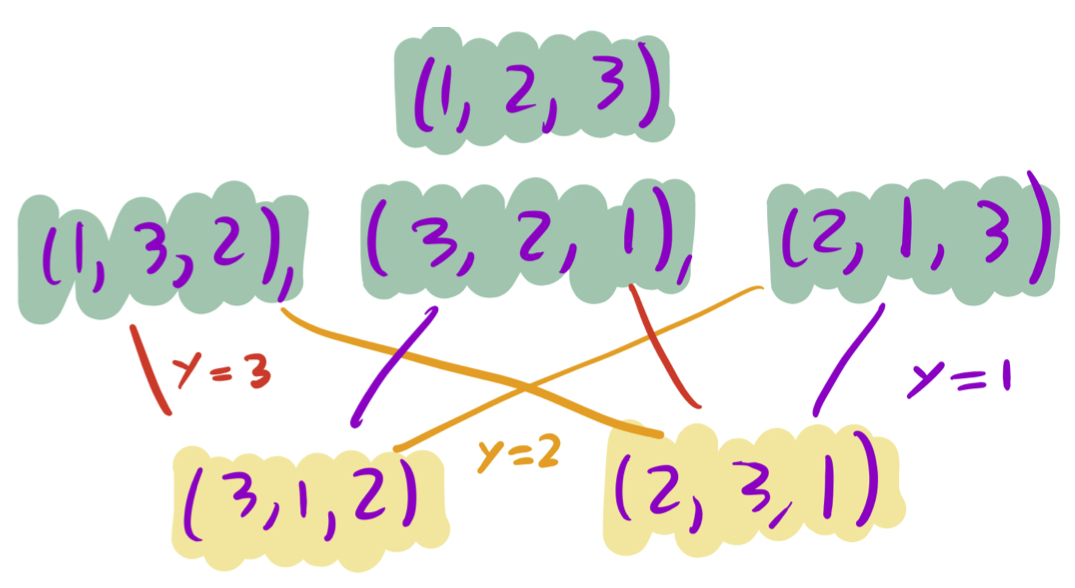
\includegraphics[height=3cm]{assets/graph.jpeg}\\
  %       & \quad f^{-1}(y) \cap g^{-1}(y) = \emptyset, \\
  %       & \quad f(x_1(y)) = g(x_1(y)), \dots, f(x_T(y)) = g(x_T(y))\}
  %     \end{align*} \pause
  %     \vspace{-2em}
  %   \item Idea 1: Study strongly non-adaptive algorithms using $G$.
  %     \pause
  %   \item Idea 2: Revisit old works  armed with shared randomness.
  %     \cite{BBSRigorousBoundsCryptanalytic2006} \inlineauthor{barkan} \inlineauthor{biham} \inlineauthor{shamir} \pause
  %     \cite{DTT10} \inlineauthor{anindya} \inlineauthor{trevisan} \inlineauthor{tulsiani}
  %   \end{itemize}
  % \end{frame}

  % \begin{frame}
  %   \frametitle{Future Directions}
  %   \begin{itemize}
  %   \item Barkan, Bihan and Shamir \nocite{BBSRigorousBoundsCryptanalytic2006} show a generic lower bound against algorithms that try to invert a random function using a ``chain-based'' strategy.
  %   \item But, by composing with random permutations, the problem of inverting an arbitrary function $f$ can be reduced to the problem of inverting a random function conditional on the same \emph{sequence of in-degrees}, that is, the same \emph{multi}-set
  %     \[[|f^{-1}(y)| : y \in [N]].\]
  %   \item This suggests that the same strategy might be able to obtain (stronger) lower bounds against chain-based algorithms that invert arbitrary functions.
  %     % Also, the bound doesn't apply to Fiat and Naor as written since the next step of each chain depends on the preprocessing.
  %   \end{itemize}
  % \end{frame}

  % \begin{frame}
  %   \frametitle{Future Directions}
  %   \begin{itemize}
  %   \item De, Trevisan and Tulsiani \nocite{DTT10} show that Fiat and Naor's tradeoff can be improved if the goal is to invert only a small fraction of inputs.
  %   \item Their work includes a new approach to analyzing Fiat and Naor's algorithm that, in hindsight, seems obviously the ``right'' approach.
  %   \item It seems plausible that this approach hasn't yet been carried to its logical conclusion. I suspect that combining it with our shared randomness lemma might lead to improving Fiat and Naor's tradeoff even when the goal is to invert all inputs.
  %   \end{itemize}
  % \end{frame}

  % \begin{frame}
  %   \frametitle{Other Work}
  %   \begin{itemize}
  %   \item Causality \inlineauthor{halpern}
  %     \pause
  %       \begin{itemize}
  %       \item \textcolor{OliveGreen}{Causal Modeling with Infinitely Many Variables}%
  %         \only<2->{\footnote{With Joe Halpern, Arxiv preprint \cite{PH21} \qquad \qquad \; \; \textcolor{OliveGreen}{Green: Finished}}}
  %         \pause
  %       \item \textcolor{OliveGreen}{Reasoning about Causal Models with Infinitely Many Variables}%
  %         \only<3->{\footnote{With Joe Halpern, appearing in AAAI'22 \cite{HP21} \qquad \textcolor{orange}{Orange: In Progress}}}
  %       \end{itemize}
  %       % selective sampling?
  %       \pause
  %     \item \textcolor{OliveGreen}{Search to Decision Reductions for Approximate Optimization}%
  %       \only<4->{\footnote{With Noah, Siyao, and Sasha, ECCC preprint \cite{S2DPreprint}}}
  %       \pause
  %   \item Lattice Algorithms
  %     \pause
  %     \begin{itemize}
  %     \item \textcolor{orange}{Novel recursive algorithm for the approximate Shortest Vector Problem}
  %       \pause
  %     \item \textcolor{orange}{$2^{\eps n}$-time complexity results on lattice problems}
  %     \end{itemize}
  %     \pause
  %   \item Black-box models and oracles
  %     \pause
  %     \begin{itemize}
  %     \item \textcolor{orange}{Generic geometric model}
  %     \end{itemize}
  % \item I'm interested in other algorithms relevant to cryptography, especially lattice algorithms
  % \item Ongoing work: a novel recursive algorithm for the Shortest Vector Problem, and $2^{\eps n}$-time reductions between lattice problems.
  % \item Leveraging ``black-box'' (oracle) models and reductions for obtaining detailed insights into the difficulty and relative difficulty of problems.
  % \item Noah and I are both quite interested in finding a natural oracle model for accessing a lattice (basis), such that (1) important algorithms (sieving, LLL) can be implemented with little overhead, but (2) we can show that they cannot be significantly improved.
  % \item I am generally interested in algorithms relevant to cryptography. I think that ``black-box'' problems, aka oracle models, aka reductions, are some of our best tools for obtaining detailed insights into the difficulty of problems (e.g., in this talk, and in another project on search-to-decision reductions for approximate optimization, I was able to show both upper and lower bounds).
  % \item I'm particularly interested in lattice algorithms. I have ongoing work on a novel recursive algorithm for the important Shortest Vector Problem (SVP). This algorithm does not improve the state-of-the-art, but its novel structure adds to our quite limited repertoire of algorithmic ideas for SVP.
  % \item I'm also working on $2^{\eps n}$-time reductions between lattice problems.
  % \item One question Noah and I are both quite interested in is whether some oracle model for accessing a lattice (basis) exists, such that important algorithms can still be implemented, but they cannot be improved (i.e., we can show a lower bound).
  %   \end{itemize}
  % \end{frame}

  \begin{frame}
    \frametitle{Thank you!}
    % In the infamous words of... catch me outside, how bout dat?
    I'm happy to take additional questions offline. You can ping me at \texttt{sp2473@cornell.edu}.
  \end{frame}

  \begin{frame}[allowframebreaks]
    \frametitle{References}
    \bibliographystyle{alpha}
    \bibliography{fi}
  \end{frame}

  % ==== EXTRA SLIDES ====
%   \begin{frame}
%     \frametitle{Bonus: a chain}
%       \scalebox{0.6}{
%        \begin{tikzpicture}[
% xnode/.style={circle, draw=green!60, fill=green!40, thick, minimum size=1.2cm},
% ynode/.style={circle, draw=blue!50, fill=blue!30, thick, minimum size=1.2cm},
% endnode/.style={circle, draw=black!25, fill=black!10, thick, minimum size=1.2cm}
% ]
% \node[xnode] (A) at (4, 3) {$x_j$};
% \node[xnode, draw=purple] (B) at (8, 3) {$x^*$};
% \node[xnode] (C) at (12, 3) {$g(y)$};
% % \node (UPPERMISSING) at (16, 10) {};
% \node[xnode] (D) at (16, 3) {};
% \node[endnode] (E) at (20, 3) {\footnotesize $h^t(x_j)$};

% \node[ynode] (X) at (6, 0) {};
% \node[ynode, draw=purple] (Y) at (10, 0) {$y$};
% % \node (LOWERMISSING) at (14, 5) {};
% \node[ynode] (Z) at (18, 0) {};

% % \draw (A) circle (0.5cm);
% % \draw (A);
% \foreach \from\to in {A/X, B/Y, D/Z}
% \draw[-Latex] (\from) -- (\to) node[midway, above right] {$f$};



% \path (C) -- node[auto=false]{\ldots} (D);
% \path (Y) -- node[auto=false]{\ldots} (Z);

% \foreach \from\to in {X/B, Z/E}
% \draw[-Latex] (\from) -- (\to) node[midway, above left] {$g$};

% \draw[-Latex, color=purple] (Y) -- (C) node[midway, above left] {$g$};
% % \draw[-Latex] (X) -- (B) node[midway, above left] {$g$};
% % \draw[-Latex, color=purple] (Y) -- (C) node[midway, above left] {$g$};
% % \draw[-Latex, color=purple] (Z) -- (E) node[midway, above left] {$g$};


% % \foreach \from\to in {A/B, B/C}
% % \draw[-Latex] (\from) -- (\to) node[midway, above] {$h$};
% \draw[-Latex, color=purple] (A) -- (B) node[midway, above] {$h$};
% \draw[-Latex] (B) -- (C) node[midway, above] {$h$};
% \draw[-Latex, color=purple] (D) -- (E) node[midway, above] {$h$};


% % \node (CZ) at (16.25, 7.5) {};
% \node (CD1) at (13.5, 3) {};
% \node (CD2) at (14.5, 3) {};

% \foreach \from\to in {C/CD1, CD2/D}
% \draw[-Latex, color=purple] (\from) -- (\to) node[midway, above] {$h$};

% % \node (ABOVE) at (12, ) {};
% \draw[-Latex, color=purple] (E) .. controls (12, 4.5) .. (A) node[midway, above] {using $(x_j, h^t(x_j))$};

% % \node (CLOWERMISSING) at (12.5, 8.75) {};
% % \node (UPPERMISSINGZ) at (17.5, 6.25) {};

% % \draw[-Latex, color=purple] (C) -- (CLOWERMISSING) node[midway, above right] {$f$};
% % \draw[-Latex, color=purple] (UPPERMISSINGZ) -- (Z) node[midway, above right] {$f$};

% % \node (YZ) at (15, 5) {};
% % \foreach \from\to in {C}

% % \draw (1, 1) -- (2, 2)
% \end{tikzpicture}}
% \end{frame}
% \begin{frame}
%   \frametitle{Function Inversion}
%     \textbf{Given} $f: [N] \to [N]$ \newline
%     and $y \in f([N])$, \newline
%     \textbf{find} $x$ such that $f(x) = y$.
%     \unnumberedfootnote{$[N] := \{0, 1, \dots, N - 1\}$}
% \end{frame}

% \begin{frame}
%   \frametitle{Function Inversion}
%     \textbf{Given} $f: [N] \to [N]$ as a \emph{black box} \newline
%      and $y \in f([N])$, \newline
%     \textbf{find} $x$ such that $f(x) = y$.
%     \unnumberedfootnote{
%       $[N] := \{0, 1, \dots, N - 1\}$ \newline
%       \emph{black box:} all you can do is evaluate $f$ on $x$ and get $y = f(x)$.
%     }
% \end{frame}

% \begin{frame}
%   \frametitle{Function Inversion}
%     \textbf{Given} $f: [N] \to [N]$ as a \emph{black box} \newline
%     \textbf{compute} small data structure $\alpha$
%      such that for all $y \in f([N])$, \newline
%      can \textbf{find} $x$ such that $f(x) = y$
%     \unnumberedfootnote{
%       $[N] := \{0, 1, \dots, N - 1\}$ \newline
%       \emph{black box:} all you can do is evaluate $f$ on $x$ and get $y = f(x)$.
%     }
%   \end{frame}


\end{document}

% % NOTES

% Role of the ``Challenger'' confusing. It's a worst-case problem, the fact that f and y can be arbitrary is clear. The communication should be with the oracle. Also, it's not the oracle which is complicated/nonstandard here. It's the preprocessing. Still, the diagram might be useful for explaining nonadaptivity and strong nonadaptivity?

% THINK OF f AS CRYPTOGRAPHIC HASH FN (where, e.g., being able to find collisions is bad!)

% Formatting with data above arrows would be helpful...

% Also: introduce trivial algorithm before Hellmans, which you should definitely include. Not clear how you want to phrase the ``quiz''--maybe just ask them to interpolate between all queries and all data?

% Be clear about S and T being proxies for space and time. It's in the title.

% Motivating preprocessing.
% (1) Black-box problem would be silly without preprocessing.
% (2) Don't want to be chasing upper bounds for specific problems; we want our algorithm to work for everything.
% (3) Worth saying something about non-uniform/preprocessing being the right attack model in real life, Rainbow Tables used in practice, governments potentially using a lot of resources to crack some standard hash functions.


% Too many ``future directions''... can condense the second two into one sentence about revisiting some old ideas armed with shared randomness if I have to.

%%%

% Rehearse, rehearse, rehearse! Especially little explanations for things.

% Meeting with Noah:
% Questions:
% Parallelism (isn't it total nonsense?)
% Check current presentation of Fiat and Naor
% Reordering the intro
% - Motivation / informal  description of preprocessing model
% - Hellman (for random here?)
% - Model (need to think about how to motivate randomness...) Here is where can be very clear what resources S and T we care about in the talk, and that we'll be calling them ``time'' and ``space''. S is *space needed for data structure*. That's it.
% - Fiat-Naor





%%% Local Variables:
%%% mode: latex
%%% TeX-master: t
%%% End:
